\section{Results and Analysis}\label{sec:results}
\newcommand{\ciacc}{[0.583, 0.843]}
\newcommand{\cimf}{[0.436, 0.608]}


\subsection{Training}
Training took 62\,min for 3 epochs (114 optimiser steps, 3.75\,ks wall clock) with a peak of 4.28\,GB of
allocated VRAM. Fig.~\ref{fig:training} shows the curves. Validation loss was lowest after epoch~2 (0.127 vs.\
0.129 after epoch~3), but generated-output validation macro-F1 kept rising (0.348, 0.436, 0.543). We selected
the checkpoint by validation macro-F1, the metric we report, so epoch~3 was used. Token-level loss is
dominated by the evidence-ID tokens and the JSON scaffold, so it is a weak proxy for the label decision.

\begin{figure}[t]
\centering
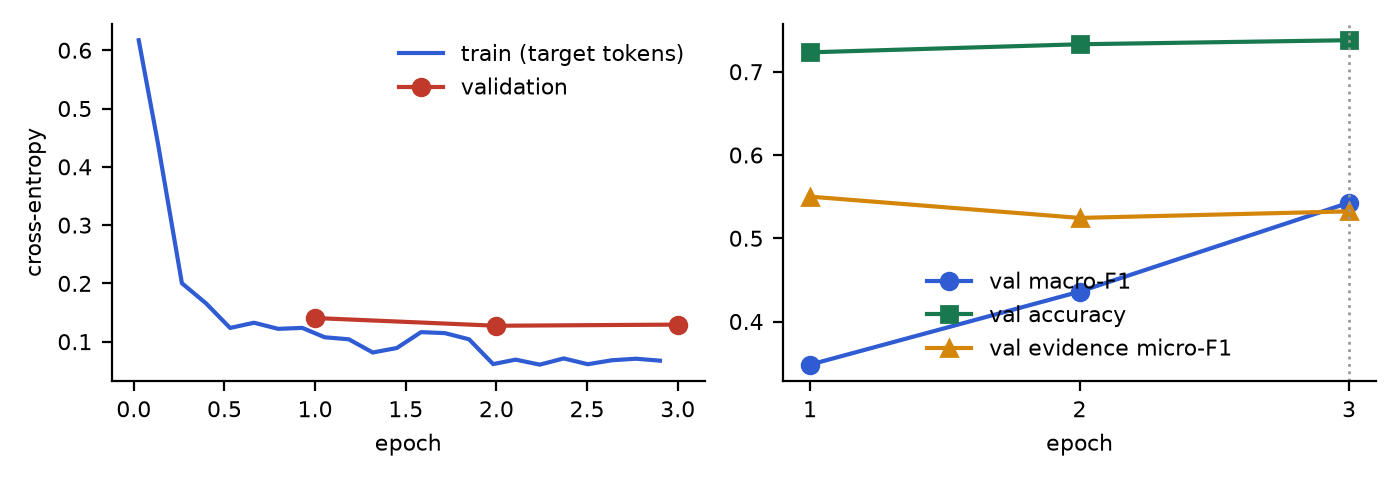
\includegraphics[width=\linewidth]{training_curves.png}
\caption{Training loss per optimiser step, and validation loss and generated-output validation macro-F1 per
epoch.}
\label{fig:training}
\end{figure}

\subsection{Classification: Before vs.\ After Fine-Tuning}
\begin{table*}[t]
\centering
\footnotesize
\caption{Same model before and after fine-tuning on identical examples (greedy, KV-cached decoder, bf16, max 64 new tokens). Macro-F1 over all 6 labels; MF1$_p$ over labels present in gold; Inc./Exc. = 4-label macro-F1 per criterion type; Ev = evidence F1; Inv = \% unparseable outputs.}
\label{tab:main}
\begin{tabular}{lrrrrrrrr}
\toprule
Model / split & Acc & MF1 & MF1$_p$ & Inc. & Exc. & Ev$_\mu$ & Ev$_M$ & Inv \\
\midrule
Base (zero-shot), val & 0.189 & 0.145 & 0.145 & 0.243 & 0.030 & 0.175 & 0.304 & 0.0 \\
Fine-tuned, val & 0.738 & 0.543 & 0.543 & 0.383 & 0.520 & 0.532 & 0.731 & 0.0 \\
\textbf{Base (zero-shot), test} & 0.160 & 0.129 & 0.155 & 0.207 & 0.042 & 0.169 & 0.354 & 0.0 \\
\textbf{Fine-tuned, test} & 0.733 & 0.440 & 0.528 & 0.425 & 0.299 & 0.561 & 0.819 & 0.0 \\
\bottomrule
\end{tabular}
\end{table*}

Table~\ref{tab:main} compares the same network with and without the adapter on identical inputs, using the
same prompt, decoder and parser. On the held-out test patients, test accuracy rose from 0.160 to 0.733
(patient-level bootstrap 95\% CI \ciacc). Macro-F1 over the labels present in gold rose from 0.155 to 0.528
(CI \cimf). Neither model produced an unparseable output, so the gain comes from label and evidence decisions,
not from formatting. The zero-shot base mostly answers \emph{included} or \emph{not applicable} and almost
never \emph{not enough information}: it treats absent facts as decisive.

Six-label macro-F1 on test (0.440) is lower than on validation (0.543) mainly because the test split contains
no \emph{excluded} example, which scores that class as~0. Over the labels present in gold the two splits agree
(0.528 vs.\ 0.543).

\begin{table}[t]
\centering
\footnotesize
\caption{Per-class results on the held-out test split (fine-tuned; base F1 for reference). Classes with zero support cannot be scored.}
\label{tab:perclass}
\begin{tabular}{llrrrrr}
\toprule
Type & Label & n & F1$_{base}$ & P & R & F1 \\
\midrule
inc. & included & 27 & 0.591 & 1.000 & 0.778 & 0.875 \\
inc. & not included & 7 & 0.000 & 0.000 & 0.000 & 0.000 \\
inc. & not enough information & 38 & 0.000 & 0.704 & 1.000 & 0.826 \\
inc. & not applicable & 3 & 0.235 & 0.000 & 0.000 & 0.000 \\
exc. & excluded & 0 & 0.000 & 0.000 & 0.000 & 0.000 \\
exc. & not excluded & 91 & 0.000 & 0.706 & 0.978 & 0.820 \\
exc. & not enough information & 28 & 0.000 & 0.000 & 0.000 & 0.000 \\
exc. & not applicable & 12 & 0.167 & 0.750 & 0.250 & 0.375 \\
\bottomrule
\end{tabular}
\end{table}

Per class (Table~\ref{tab:perclass}), the model is strong and precise on \emph{included} (P\,=\,1.00, F1 0.875)
and \emph{not excluded} (F1 0.820). It is weak on the rare classes:
\begin{itemize}
\item \emph{not included}: all 7 test cases were predicted \emph{not enough information};
\item \emph{not applicable}: recall is 0.20.
\end{itemize}
These are the classes with the fewest training examples, so the result matches the label skew documented in
Section~\ref{sec:split}. For exclusion criteria, 28 of the 66 \emph{not enough information} cases were
predicted \emph{not excluded}. This reproduces, in a milder form, the base model's habit of reading silence as
a negative finding. The confusion matrices in Fig.~\ref{fig:cm} show the same pattern.

\begin{figure}[t]
\centering
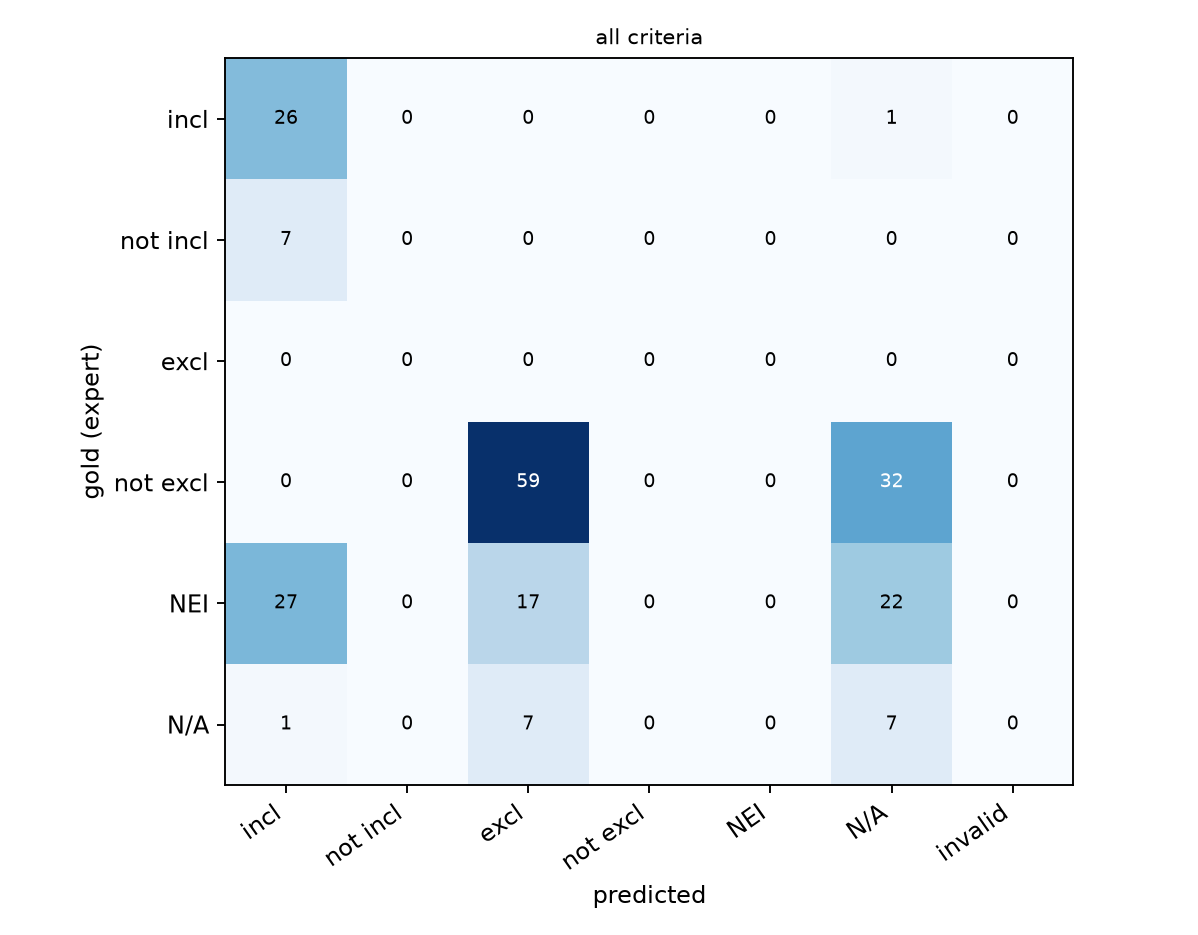
\includegraphics[width=0.49\linewidth]{cm_base_all.png}\hfill
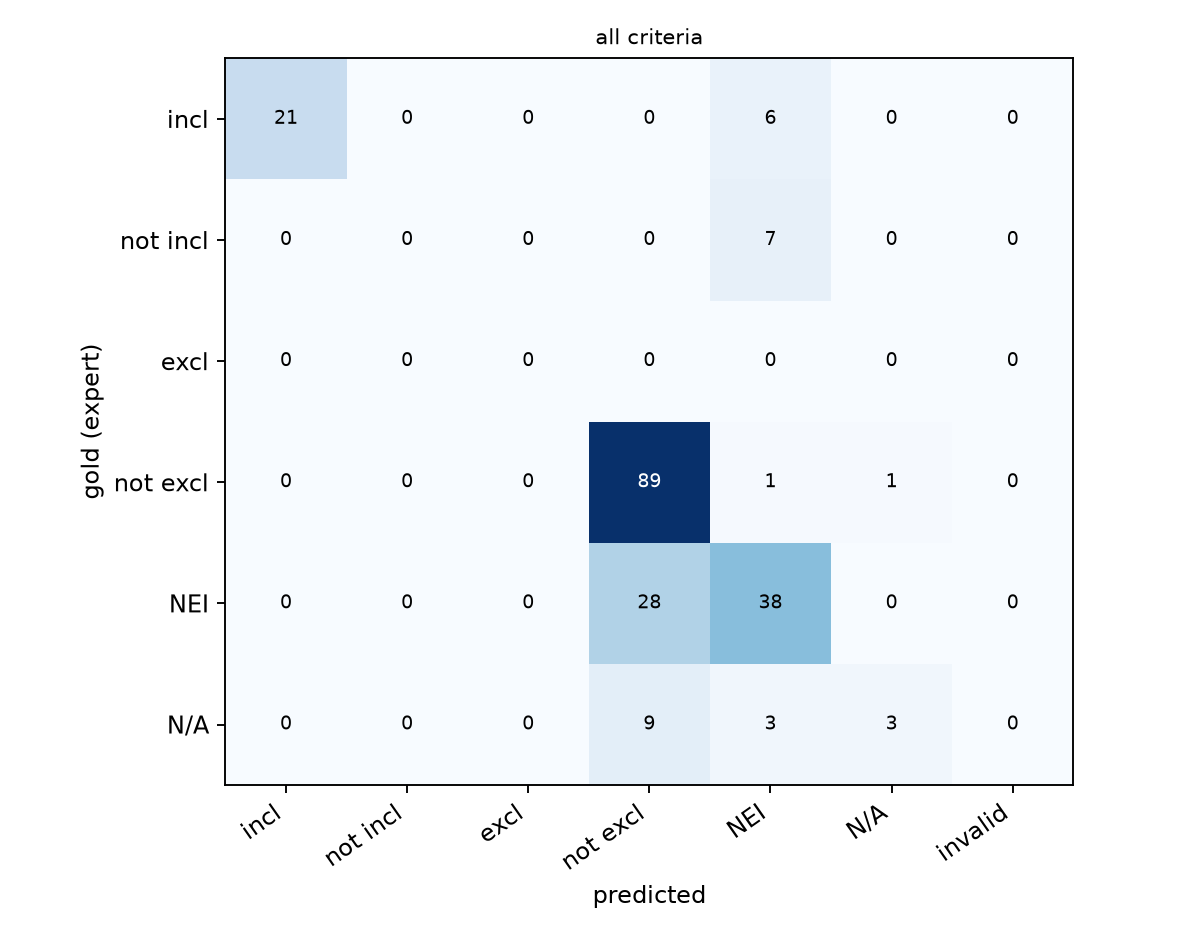
\includegraphics[width=0.49\linewidth]{cm_finetuned_all.png}
\caption{Test confusion matrices over all six labels: zero-shot base (left) and fine-tuned (right).}
\label{fig:cm}
\end{figure}

\subsection{Evidence Retrieval}
\begin{table*}[t]
\centering
\footnotesize
\caption{Evidence-sentence retrieval on the test split. Micro pools TP/FP/FN; macro averages per record (both-empty = 1, see Sec.~\ref{sec:metrics}). NE = non-empty-gold subset; Abst. = correct empty predictions for empty gold; Uns. = cited IDs not in the note.}
\label{tab:evidence}
\begin{tabular}{lrrrrrrrrr}
\toprule
Model & P$_\mu$ & R$_\mu$ & F1$_\mu$ & P$_M$ & R$_M$ & F1$_M$ & F1$_{NE}$ & Abst. & Uns. \\
\midrule
Base & 0.097 & 0.649 & 0.169 & 0.374 & 0.899 & 0.354 & 0.374 & 53/145 & 0 \\
Fine-tuned & 0.500 & 0.638 & 0.561 & 0.888 & 0.904 & 0.819 & 0.663 & 131/145 & 0 \\
\bottomrule
\end{tabular}
\end{table*}

Fine-tuning improves evidence citation more than any other metric (Table~\ref{tab:evidence}). Micro-F1 rose
from 0.169 to 0.561, and the gain came almost entirely from precision (0.097 to 0.500), with recall unchanged
(0.649 vs.\ 0.638). The base model cites many sentences indiscriminately. The fine-tuned model abstains
correctly on 131 of the 145 empty-gold criteria, compared with 53 for the base model. On the non-empty-gold
subset, which isolates retrieval from abstention, F1 rose from 0.374 to 0.663. Neither model cited a sentence
ID outside the note.

\begin{figure*}[t]
\centering
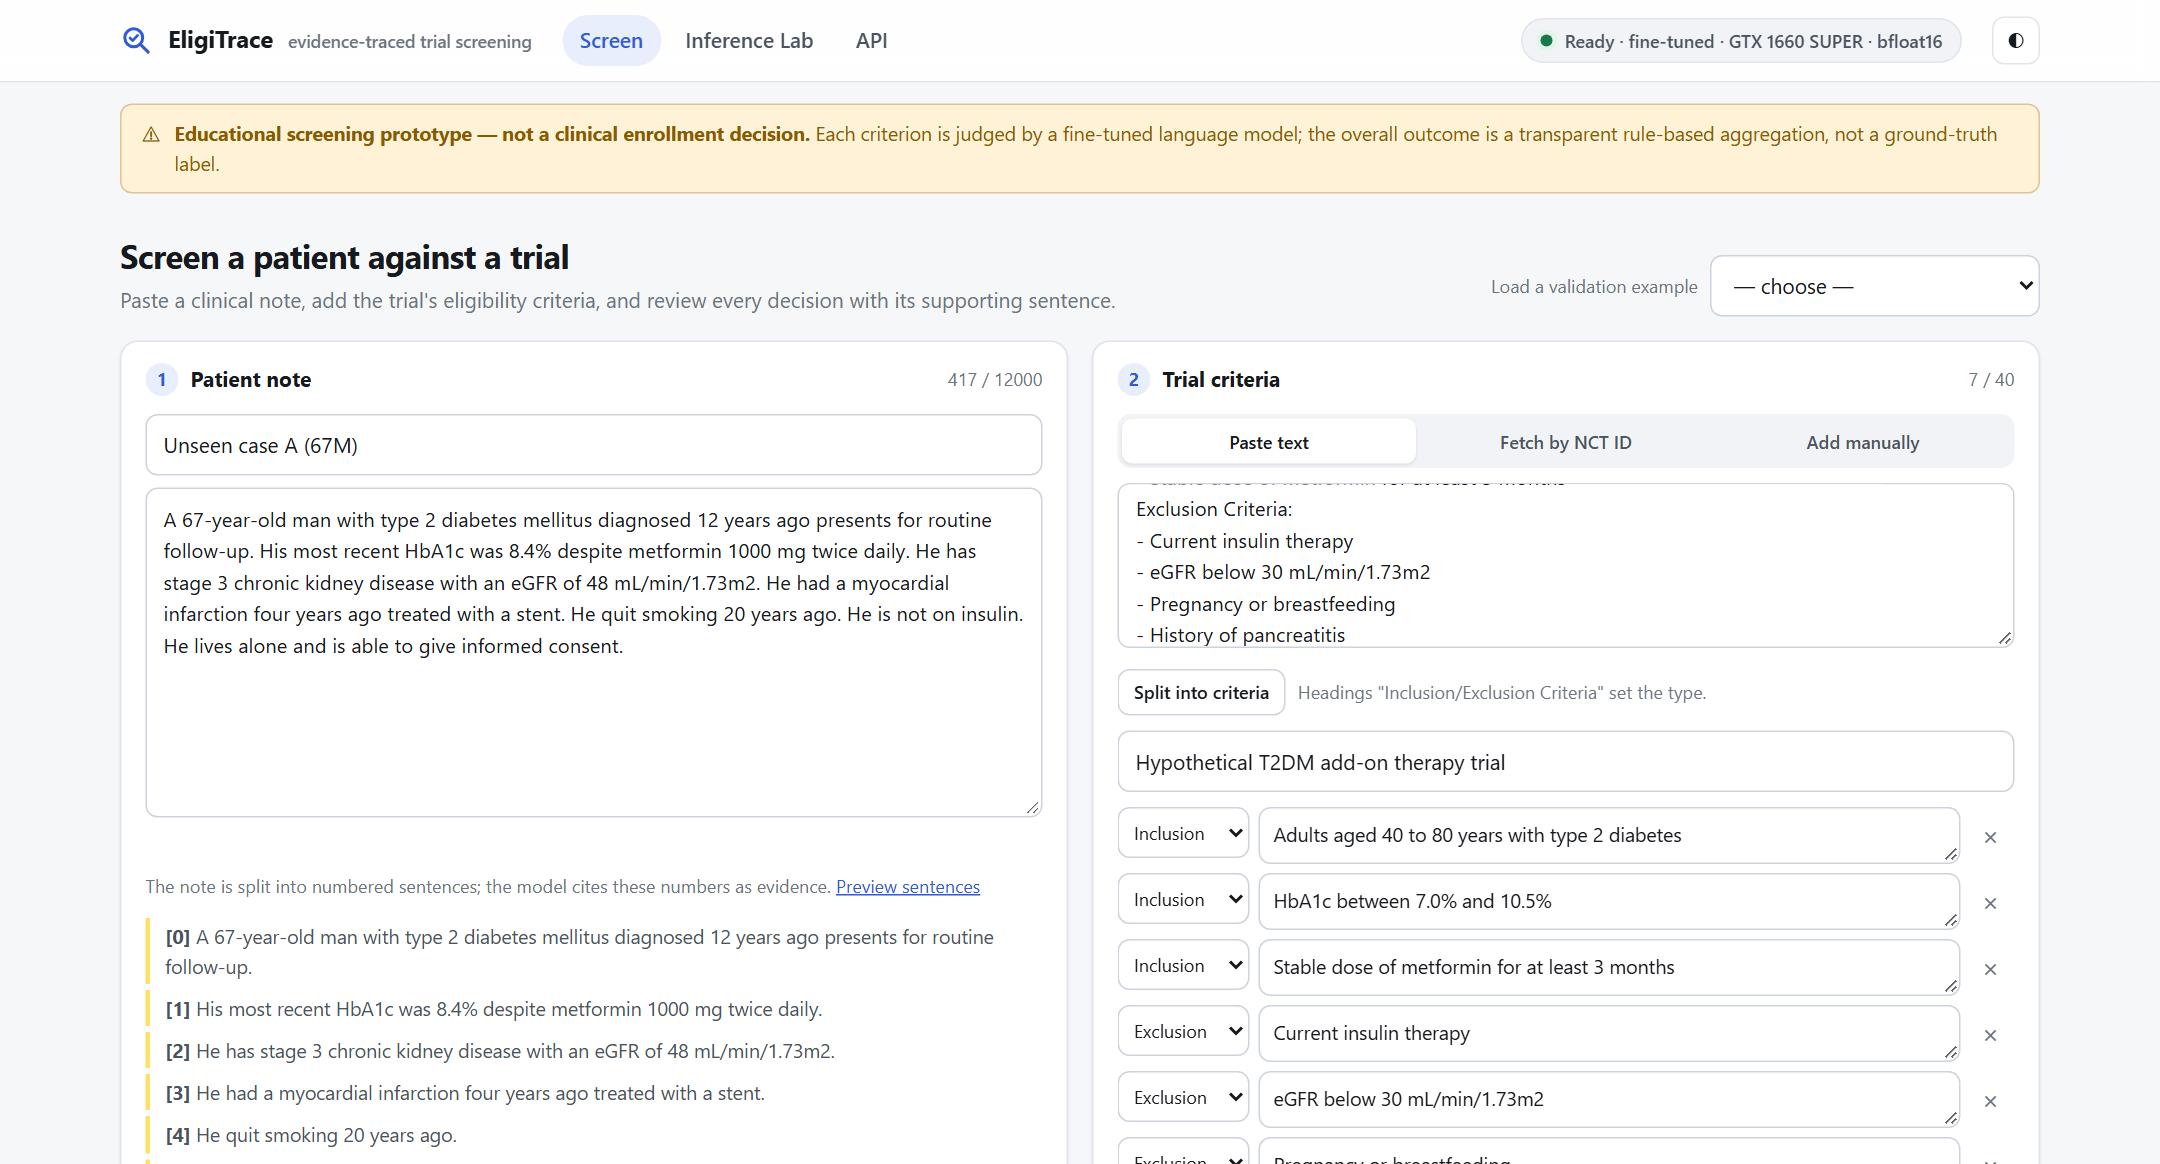
\includegraphics[width=0.49\linewidth]{screens/02_input_top.png}\hfill

\includegraphics[width=0.49\linewidth]{screens/03_results_top.png}\\[4pt]
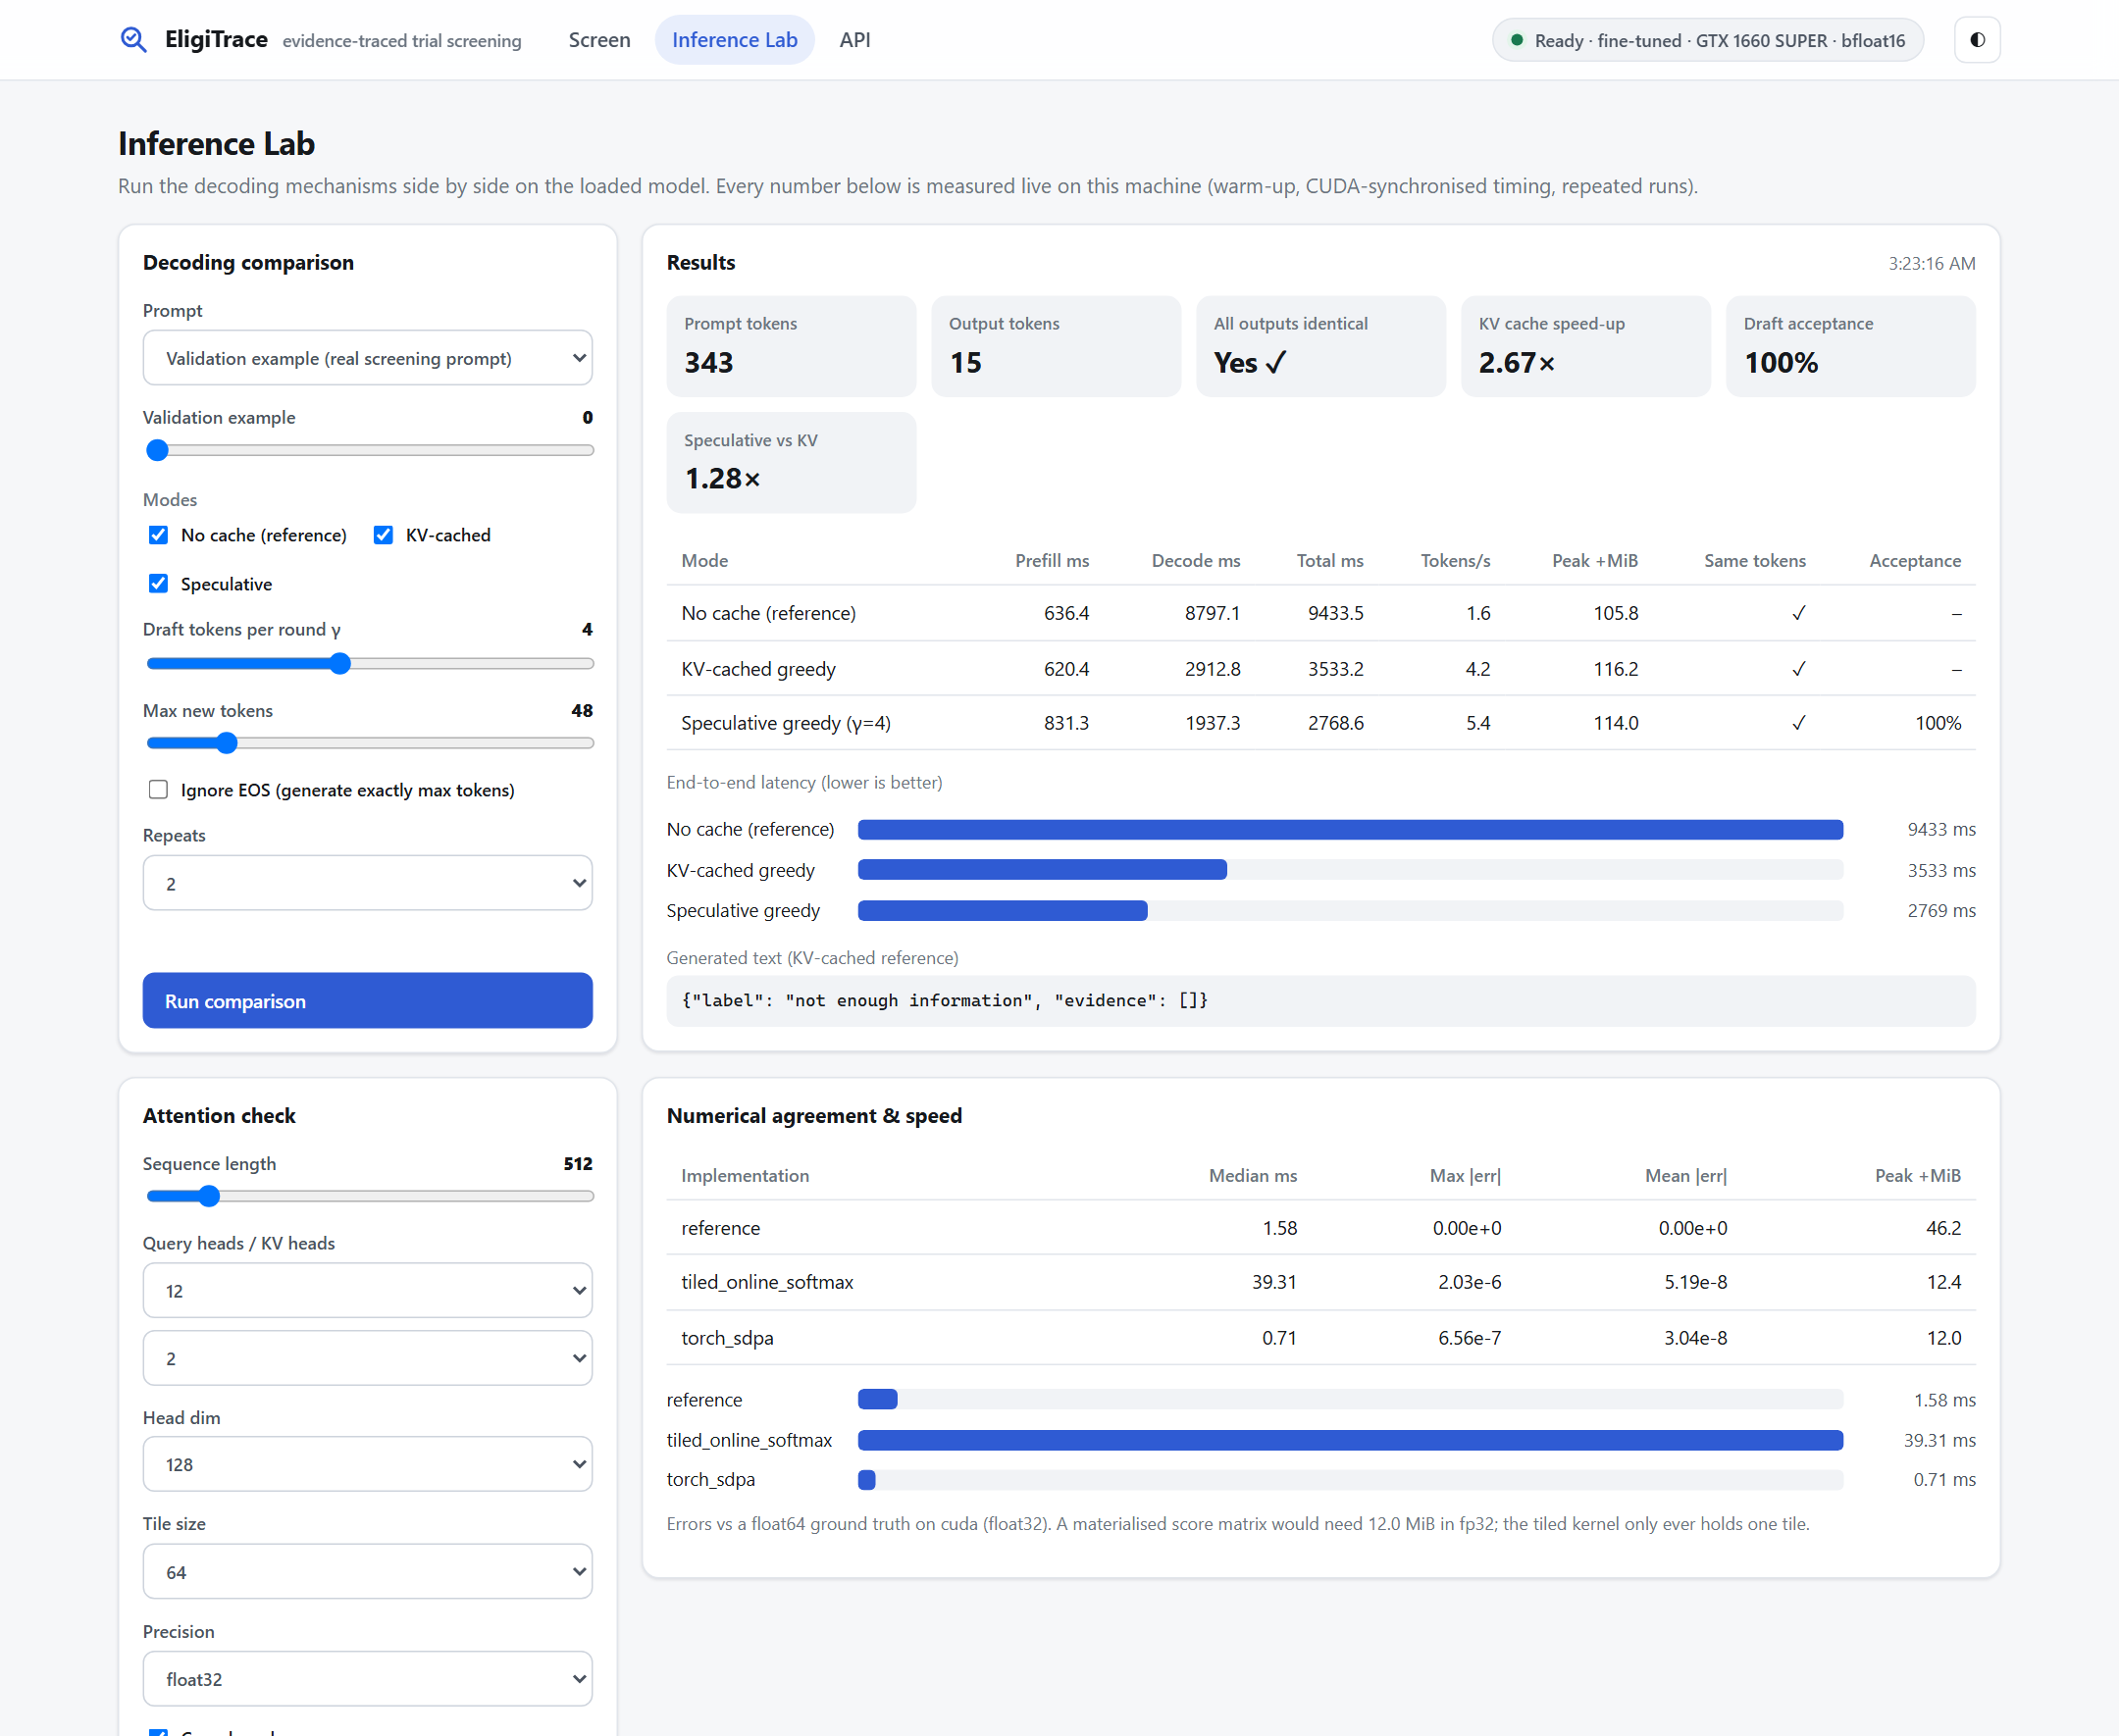
\includegraphics[width=0.49\linewidth]{screens/06_lab.png}\hfill
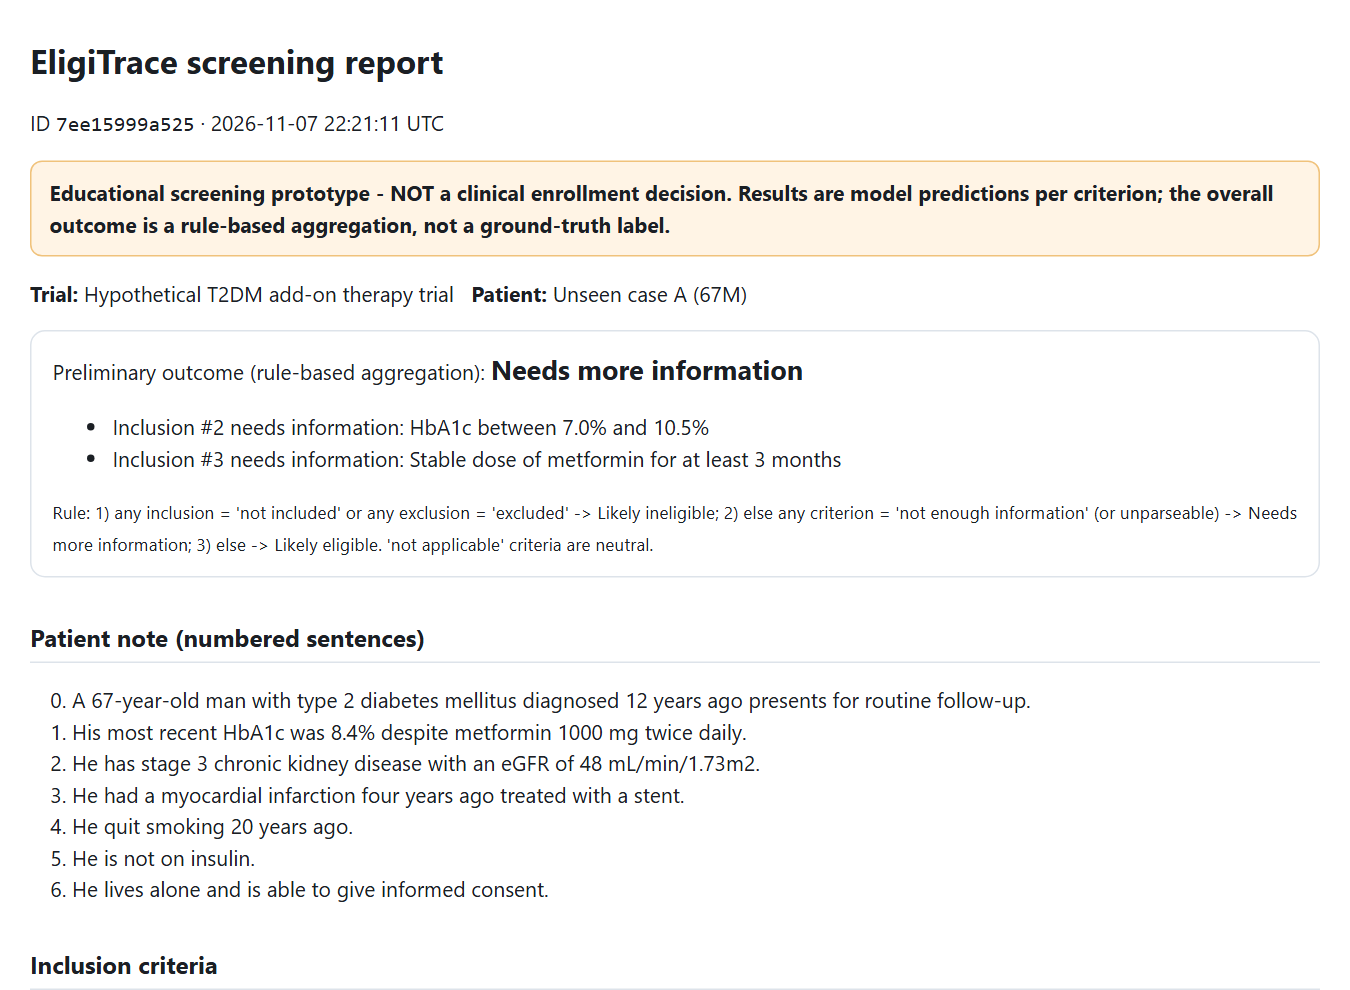
\includegraphics[width=0.49\linewidth]{screens/04_report_top.png}
\caption{\sys\ application. Top: input of an unseen note and criteria (left), and criterion results with
highlighted evidence, grounded rationales and the rule-based outcome (right). Bottom: Inference Lab with live
decoder and attention comparisons (left), and the exported report with provenance (right).}
\label{fig:app}
\end{figure*}

\subsection{Error Analysis}
\begin{table}[t]
\centering
\footnotesize
\caption{Rule-assigned error categories, fine-tuned model, test split (55 wrong labels of 206; one error may have several).}
\label{tab:errors}
\begin{tabular}{lr}
\toprule
Category & Count \\
\midrule
correct label, wrong evidence & 34 \\
missing information treated as decisive (unsupported decision) & 28 \\
temporal qualifier & 19 \\
false 'not enough information' (evidence was present) & 17 \\
not-applicable confusion & 13 \\
negation in evidence & 7 \\
numeric / threshold reasoning & 6 \\
cited evidence where experts found none & 3 \\
\bottomrule
\end{tabular}
\end{table}

Of the 206 test criteria, 55 received the wrong label. Table~\ref{tab:errors} groups them with deterministic
rules (\texttt{evaluation/errors.py}). The most frequent pattern is an unsupported decision, where missing
information is treated as decisive (28 cases). Temporal qualifiers such as ``within the past 6 months'' and
``history of'' are next (19 cases). The opposite error, answering \emph{not enough information} although the
experts found the note sufficient, occurs 17 times.

One instructive case is a vascular-surgery trial whose inclusion criteria list specific operations
(``patients undergoing open abdominal aortic aneurysm repair''). For a patient with a femoral pseudoaneurysm,
the experts labelled these criteria \emph{not included} with no evidence: a note that describes a different
procedure implies the listed one is not happening. The model answered \emph{not enough information} and cited
the three sentences describing the actual procedure. Expert reasoning of this kind rests on the absence of a
fact in an otherwise complete clinical picture, and it is underrepresented in 603 training examples.

A further 34 records have the correct label but differ from the gold evidence. Most of these are omissions on
\emph{not excluded} criteria, where the annotators cited background sentences such as the demographic opening
line.

\subsection{KV-Cached Decoding}\label{sec:res-kv}
\begin{table*}[t]
\centering
\footnotesize
\caption{KV-cached vs.\ no-cache greedy decoding (fine-tuned target, bf16, batch 1, EOS disabled; mean of 3 synchronised runs after 1 warm-up). Peak = extra MiB over resident weights. Eq. = token-identical output.}
\label{tab:kv}
\begin{tabular}{rrrrrrrrrrc}
\toprule
In & Out & Pre ms & Dec ms & tok/s & Dec ms$_{nc}$ & tok/s$_{nc}$ & Speed-up & Peak & Peak$_{nc}$ & Eq. \\
\midrule
128 & 16 & 189 & 1098 & 12.4 & 3810 & 4.0 & 3.5 & 44 & 42 & no@5 \\
128 & 64 & 216 & 4546 & 13.4 & 16357 & 3.9 & 3.6 & 44 & 57 & no@5 \\
128 & 128 & 228 & 10014 & 12.5 & 38493 & 3.3 & 3.8 & 44 & 75 & no@5 \\
512 & 16 & 653 & 1084 & 9.2 & 10882 & 1.4 & 10.0 & 172 & 154 & yes \\
512 & 64 & 667 & 4570 & 12.2 & 45849 & 1.4 & 10.0 & 172 & 168 & yes \\
512 & 128 & 683 & 9163 & 13.0 & 98547 & 1.3 & 10.8 & 172 & 188 & yes \\
1024 & 16 & 1380 & 1151 & 6.3 & 21827 & 0.7 & 19.0 & 346 & 305 & yes \\
1024 & 64 & 1382 & 5026 & 10.0 & 89785 & 0.7 & 17.9 & 346 & 319 & yes \\
1024 & 128 & 1352 & 9326 & 12.0 & 186221 & 0.7 & 20.0 & 346 & 337 & no@84 \\
\bottomrule
\end{tabular}
\end{table*}

Table~\ref{tab:kv} and Fig.~\ref{fig:kv} compare the two decoders. Prefill cost is the same for both, since
both process the prompt once. Without a cache, every decode step reprocesses the whole sequence, so no-cache
throughput falls from 4.0 to 0.7\,tok/s as the input grows from 128 to 1024 tokens. With the cache, each step
costs one token through the network and throughput stays between 9 and 13\,tok/s. Decode speed-up therefore
grows with context: about $3.6\times$ at 128 input tokens, $10\times$ at 512 and $18$--$20\times$ at 1024.

Peak extra memory is dominated by prefill activations (the $T\times151{,}936$ logit matrix), not by the cache.
The cache adds 28\,KiB per token, so it occupies only 32\,MiB even at 1{,}152 tokens. At batch~1 on this GPU,
decoding is launch-bound: a single-token step costs about 75--110\,ms whatever the context length, which is
why the cached throughput stays flat.

\begin{figure}[t]
\centering
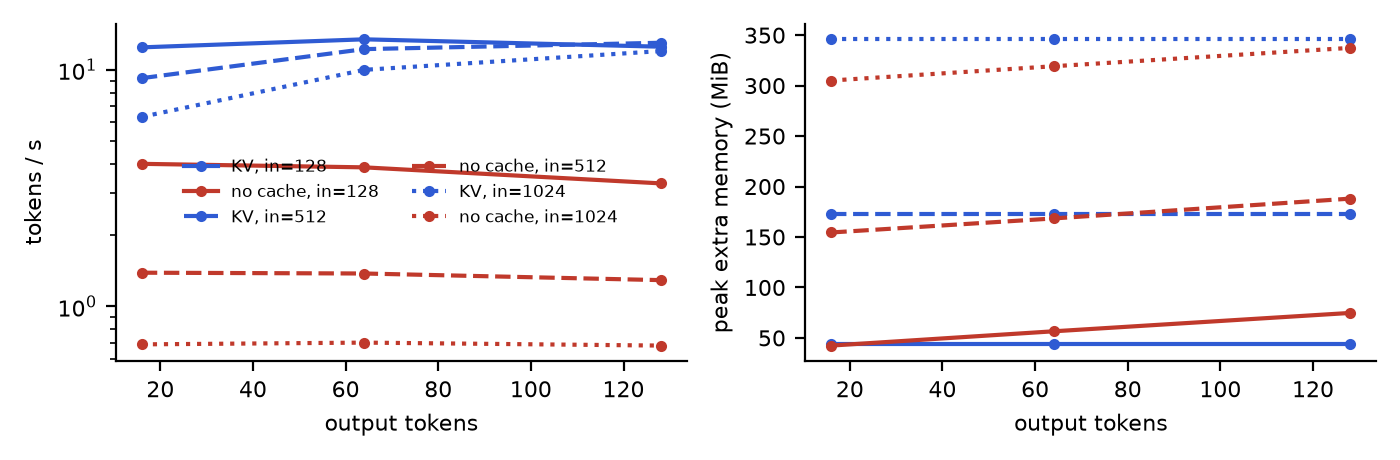
\includegraphics[width=\linewidth]{kv_benchmark.png}
\caption{Decode throughput (left) and peak extra memory (right) of the KV-cached decoder and the no-cache reference vs.\ input and output length.}
\label{fig:kv}
\end{figure}

\textbf{Equality.} The CPU fp64 tests on tiny Qwen2 models and the bf16 GPU test on the base model produce
token-identical output for both decoders. With the merged fine-tuned weights in bf16, 6 of the 9 benchmark
cases are identical. The other three diverge at a step where the top-2 logit margin is 0.125, which is exactly
one bf16 unit in the last place for logits between 16 and 32. In other words, the two candidate tokens are
tied at bf16 resolution. The cached path computes attention for one query against stored keys, while the
reference recomputes the full $T\times T$ product; the two reduction orders round differently, and a tie can
go either way. Section~\ref{sec:res-numerics} tests this explanation in fp32.

\subsection{Tiled Attention}
\begin{table}[t]
\centering
\footnotesize
\caption{Attention agreement with a float64 reference over the validation grid (3 head layouts incl.\ GQA 12:2, 8 $(S_q,S_k)$ shapes incl.\ decode $S_q{=}1$, $d\in\{32,64,128\}$, causal on/off; tiled also over tile sizes 16/64/128).}
\label{tab:attnerr}
\begin{tabular}{llrrr}
\toprule
Impl. & dtype & Cases & max $|\Delta|$ & mean $|\Delta|$ \\
\midrule
reference & bfloat16 & 144 & 7.80e-03 & 1.83e-04 \\
reference & float16 & 144 & 9.76e-04 & 2.28e-05 \\
reference & float32 & 144 & 0.00e+00 & 0.00e+00 \\
tiled & bfloat16 & 432 & 7.80e-03 & 1.83e-04 \\
tiled & float16 & 432 & 9.76e-04 & 2.28e-05 \\
tiled & float32 & 432 & 2.74e-06 & 2.82e-08 \\
torch\_sdpa & bfloat16 & 144 & 7.80e-03 & 1.83e-04 \\
torch\_sdpa & float16 & 144 & 9.76e-04 & 2.28e-05 \\
torch\_sdpa & float32 & 144 & 2.38e-06 & 2.63e-08 \\
\bottomrule
\end{tabular}
\end{table}

Against a float64 ground truth, the tiled kernel matches PyTorch SDPA to the precision of its storage format
(Table~\ref{tab:attnerr}). In fp32 its maximum error is $2.7\times10^{-6}$ against $2.4\times10^{-6}$ for SDPA,
over 432 cases that cover GQA (12:2), decode shapes with $S_q{=}1$, causal and non-causal masks, and tile sizes
16, 64 and 128. In bf16 and fp16 all three implementations have the same error, set by rounding the output to
the storage type.

Speed and memory show the expected trade-off (Fig.~\ref{fig:attn}). On the GTX~1660 SUPER (sm\_75), PyTorch's
fused flash and memory-efficient kernels are unavailable in bf16, so the fair baseline is the unfused
\texttt{math} backend. At sequence length 4096, that backend materialises the score matrix and needs 1.9\,GB of
extra memory, whereas the tiled kernel needs 41\,MiB, about 46$\times$ less. Being a Python loop over tiles, the
tiled kernel is slower: 465\,ms vs.\ 73\,ms with 128-wide tiles. Larger tiles reduce the number of kernel
launches and run $3.7\times$ faster than 64-wide tiles. This is the I/O-versus-launch trade-off that fused
kernels such as FlashAttention remove~\cite{dao2022flashattention}.

\begin{figure}[t]
\centering
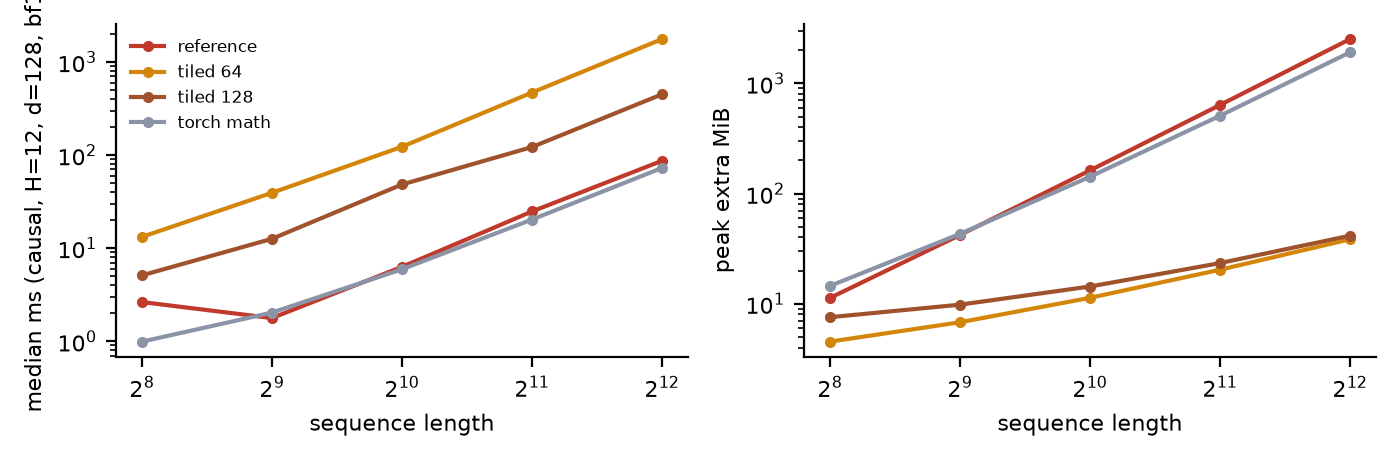
\includegraphics[width=\linewidth]{attention_benchmark.png}
\caption{Attention latency and peak extra memory vs.\ sequence length (bf16, GPU, 12 query / 2 KV heads,
$d$=128, causal).}
\label{fig:attn}
\end{figure}

\subsection{Speculative Decoding}
\begin{table*}[t]
\centering
\footnotesize
\caption{Greedy speculative decoding (target: fine-tuned Qwen2.5-1.5B, draft: Qwen2.5-0.5B, bf16) vs.\ KV-cached greedy on the same 8 validation prompts. Acc.\ = accepted/proposed; $\bar n$ = accepted per round; Fwd/tok = target forwards per output token.}
\label{tab:spec}
\begin{tabular}{lrrrrrrrc}
\toprule
Workload & $\gamma$ & Lat. ms & tok/s & Acc. & $\bar n$ & Fwd/tok & Speed-up & Eq. \\
\midrule
task\_json & greedy & 1437 & 9.9 & -- & -- & 1.00 & 1.00 & yes \\
task\_json & 1 & 2089 & 6.8 & 0.91 & 0.91 & 0.58 & 0.69 & yes \\
task\_json & 2 & 2190 & 6.5 & 0.71 & 1.43 & 0.48 & 0.66 & yes \\
task\_json & 3 & 2296 & 6.3 & 0.60 & 1.80 & 0.43 & 0.63 & no \\
task\_json & 4 & 2279 & 6.3 & 0.59 & 2.35 & 0.37 & 0.63 & yes \\
task\_json & 6 & 2420 & 5.9 & 0.51 & 3.04 & 0.32 & 0.59 & yes \\
task\_json & 8 & 2767 & 5.1 & 0.40 & 3.22 & 0.31 & 0.52 & yes \\
free\_96 & greedy & 7345 & 13.1 & -- & -- & 1.00 & 1.00 & yes \\
free\_96 & 1 & 11392 & 8.4 & 0.76 & 0.76 & 0.58 & 0.64 & no \\
free\_96 & 2 & 11730 & 8.2 & 0.61 & 1.21 & 0.46 & 0.63 & no \\
free\_96 & 3 & 12251 & 7.8 & 0.55 & 1.62 & 0.39 & 0.60 & no \\
free\_96 & 4 & 13105 & 7.3 & 0.48 & 1.90 & 0.35 & 0.56 & no \\
free\_96 & 6 & 13899 & 6.9 & 0.44 & 2.59 & 0.29 & 0.53 & no \\
free\_96 & 8 & 18911 & 5.1 & 0.29 & 2.25 & 0.32 & 0.39 & no \\
\bottomrule
\end{tabular}
\end{table*}

The draft and target models share tokenizer, special tokens and chat template, which we verified
programmatically. Acceptance is high: 91\% of drafted tokens are accepted at $\gamma{=}1$ on the
structured-output task, and acceptance falls to 40\% at $\gamma{=}8$ (Table~\ref{tab:spec}, Fig.~\ref{fig:spec}).
The number of target forwards per output token falls from 1.0 to 0.31.

Even so, speculative decoding was \emph{slower} than KV-cached greedy decoding at every $\gamma$, at
0.39--0.69$\times$ its speed. The reason is that at batch~1 on this GPU, forward cost scales with the number of
layers and kernel launches rather than with parameter count. The 0.5B draft has 24 layers against the target's
28, so a draft step costs almost as much as a target step. We timed this directly, with greedy cached decoding
after a 512-token prompt in bf16: one draft step took 189\,ms and one target step took 239\,ms, a ratio of
0.79, although the draft has a third of the target's parameters. Saving a target forward therefore saves less time
than the extra draft steps add. Speculative decoding pays off when the draft is much cheaper per token than the
target, for example a larger target, a shallower draft, or a compute-bound regime. We report the negative
result as measured.

\begin{figure}[t]
\centering
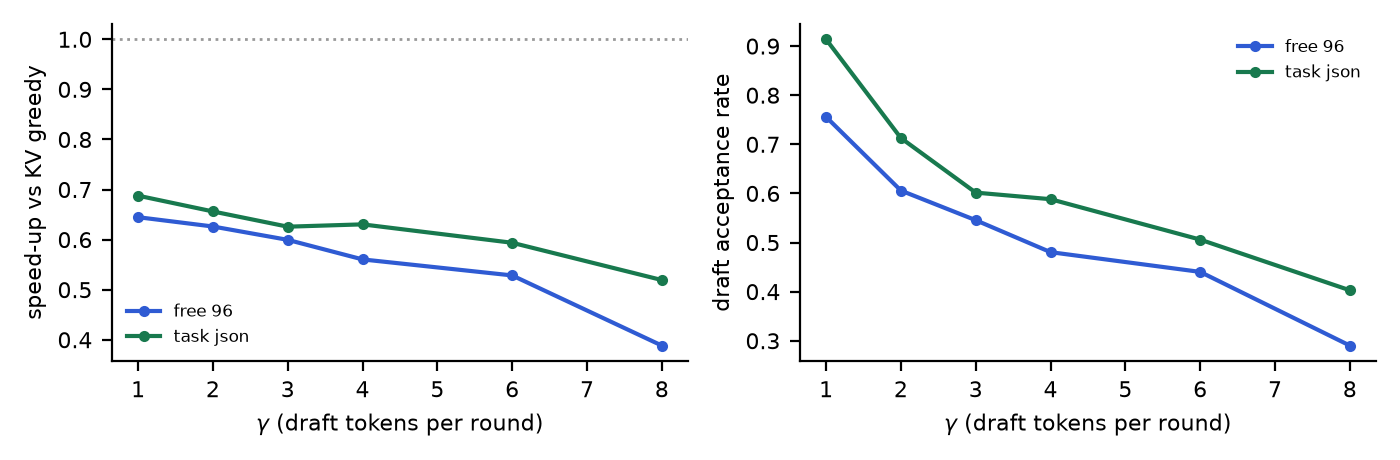
\includegraphics[width=\linewidth]{spec_benchmark.png}
\caption{Speculative decoding: acceptance rate and speed-up over KV-cached greedy decoding vs.\ draft length
$\gamma$.}
\label{fig:spec}
\end{figure}

\subsection{Numerical Agreement in bf16 vs.\ fp32}\label{sec:res-numerics}
All three mechanisms are exact in exact arithmetic, yet each produced a few bf16 outputs that differ from its
reference. We checked whether these differences come from bugs or from rounding, using
\texttt{speculative/investigate.py}, \texttt{attention/hf\_integration.py} and \texttt{kvcache/fp32\_check.py}.

\textbf{Margins at the divergence point.} Every bf16 divergence we found occurs where the two best logits
differ by at most 0.125. For logits in $[16,32)$, the spacing between adjacent bf16 values is $2^{4-7}=0.125$,
so the two tokens are tied, or one rounding step apart. For speculative example~0, the target logits at
step~22 are 18.375 vs.\ 18.25 when tokens are processed one at a time, as in greedy decoding. Inside the
5-token verification block used by speculative decoding, the same two logits come out \emph{exactly equal}
(17.875 and 17.875), and the tie is broken the other way. The single-token and block paths differ by up to 0.84
in individual logits. Different matrix shapes select different GEMM kernels and reduction orders, and bf16
keeps only 8 bits of mantissa.

\textbf{fp32 reruns.} Table~\ref{tab:fp32} repeats the diverging cases in fp32 on the CPU, without changing any
code. Speculative decoding then matches greedy decoding token for token on all three investigated prompts.
With the tiled kernel substituted for every attention layer of the fine-tuned model through the Transformers
\texttt{AttentionInterface}, final-position logits stay within $3.4\times10^{-4}$ of SDPA. Greedy output is
identical on all three prompts, whereas in bf16 the logit gap is 0.5--0.7 and one prompt diverges.
Finally, the KV-cached decoder matches the no-cache reference in fp32 on both bf16-diverging KV cases: (128 in,
16 out), which diverged at step~5, and (1024 in, 128 out), which diverged at step~84. The fp32 runs took
59\,min on the CPU, mostly in the quadratic no-cache reference.

\begin{table}[t]
\centering
\footnotesize
\caption{Token agreement with the reference in bf16 (GPU) vs.\ fp32 (CPU), on the cases that diverged in
bf16.}
\label{tab:fp32}
\begin{tabular}{lcc}
\toprule
Check & bf16 GPU & fp32 CPU \\
\midrule
Speculative vs.\ greedy ($\gamma{=}4$, 3 prompts) & 1/3 equal & 3/3 equal \\
Tiled attention in model vs.\ SDPA (3 prompts) & 2/3 equal & 3/3 equal \\
\quad max $|\Delta\text{logit}|$ & 0.70 & $3.4\times10^{-4}$ \\
KV-cached vs.\ no-cache (2 diverging cases) & 0/2 equal & 2/2 equal \\
\bottomrule
\end{tabular}
\end{table}

The mechanisms are therefore exact. In bf16 they are reproducible only up to ties within one rounding step,
which is also true of production inference stacks. Any bf16 equality claim should be read with that caveat.


\subsection{Application}\label{sec:res-app}
Fig.~\ref{fig:app} shows the running application, served on the same GPU used for evaluation. Each test used a
note that is not in the dataset, together with criteria that we wrote ourselves:
\begin{itemize}
\item a 67-year-old man with type~2 diabetes and stage~3 chronic kidney disease;
\item a hypothetical add-on therapy trial with three inclusion and four exclusion criteria.
\end{itemize}
The note is split into numbered sentences, and each criterion is decoded and displayed as soon as it finishes.
Each result card shows:
\begin{itemize}
\item the label, with both criterion types kept and all expert categories preserved;
\item the cited sentences, which are also highlighted in the note;
\item a rationale that passed the grounding check, or the deterministic template when it did not.
\end{itemize}
The overall outcome is shown together with the rule that produced it.

Invalid input is rejected with a field-level message and the user's draft is kept. This covers empty notes,
malformed NCT IDs and unknown labels. An unreachable ClinicalTrials.gov service or a model that is still
loading returns a clear message, not a stack trace.

The Inference Lab runs the no-cache, KV-cached and speculative decoders on the loaded model. For each run it
reports timing, token equality and draft acceptance, and it also runs the attention check against a float64
ground truth.

\begin{figure*}[t]
\centering
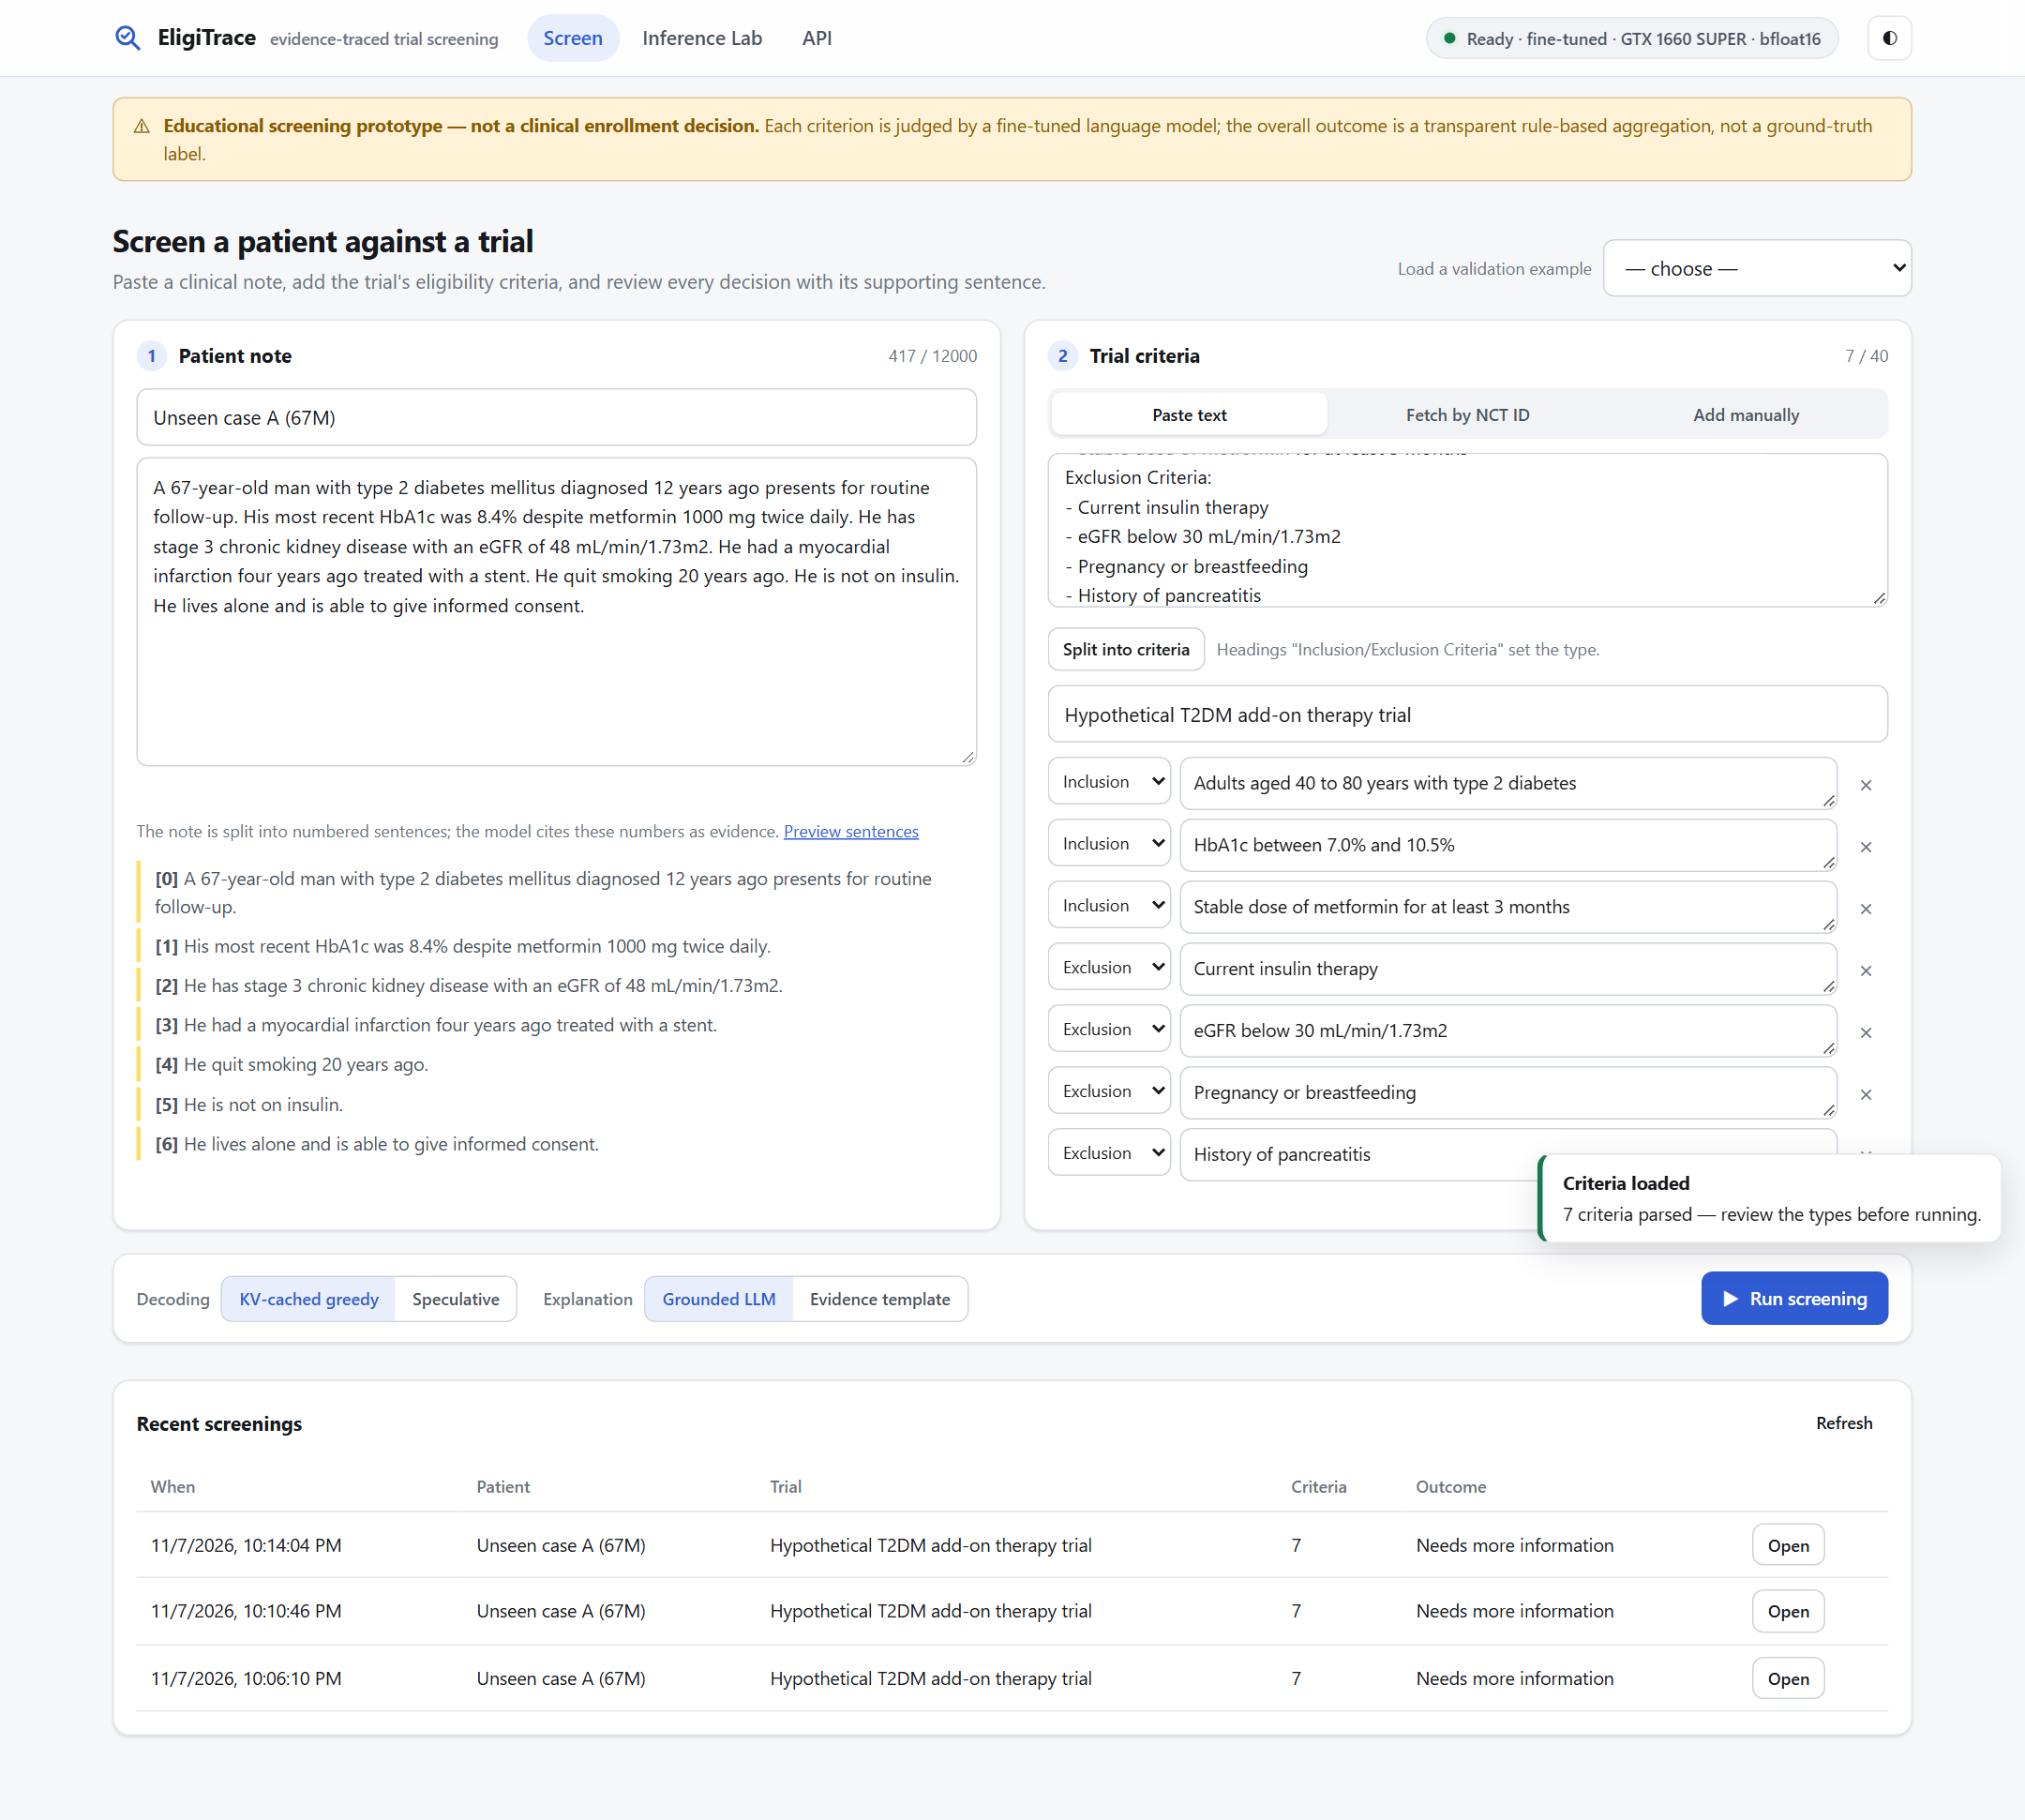
\includegraphics[width=0.49\linewidth]{screens/02_input.png}\hfill

\includegraphics[width=0.49\linewidth]{screens/03_results.png}\\[4pt]
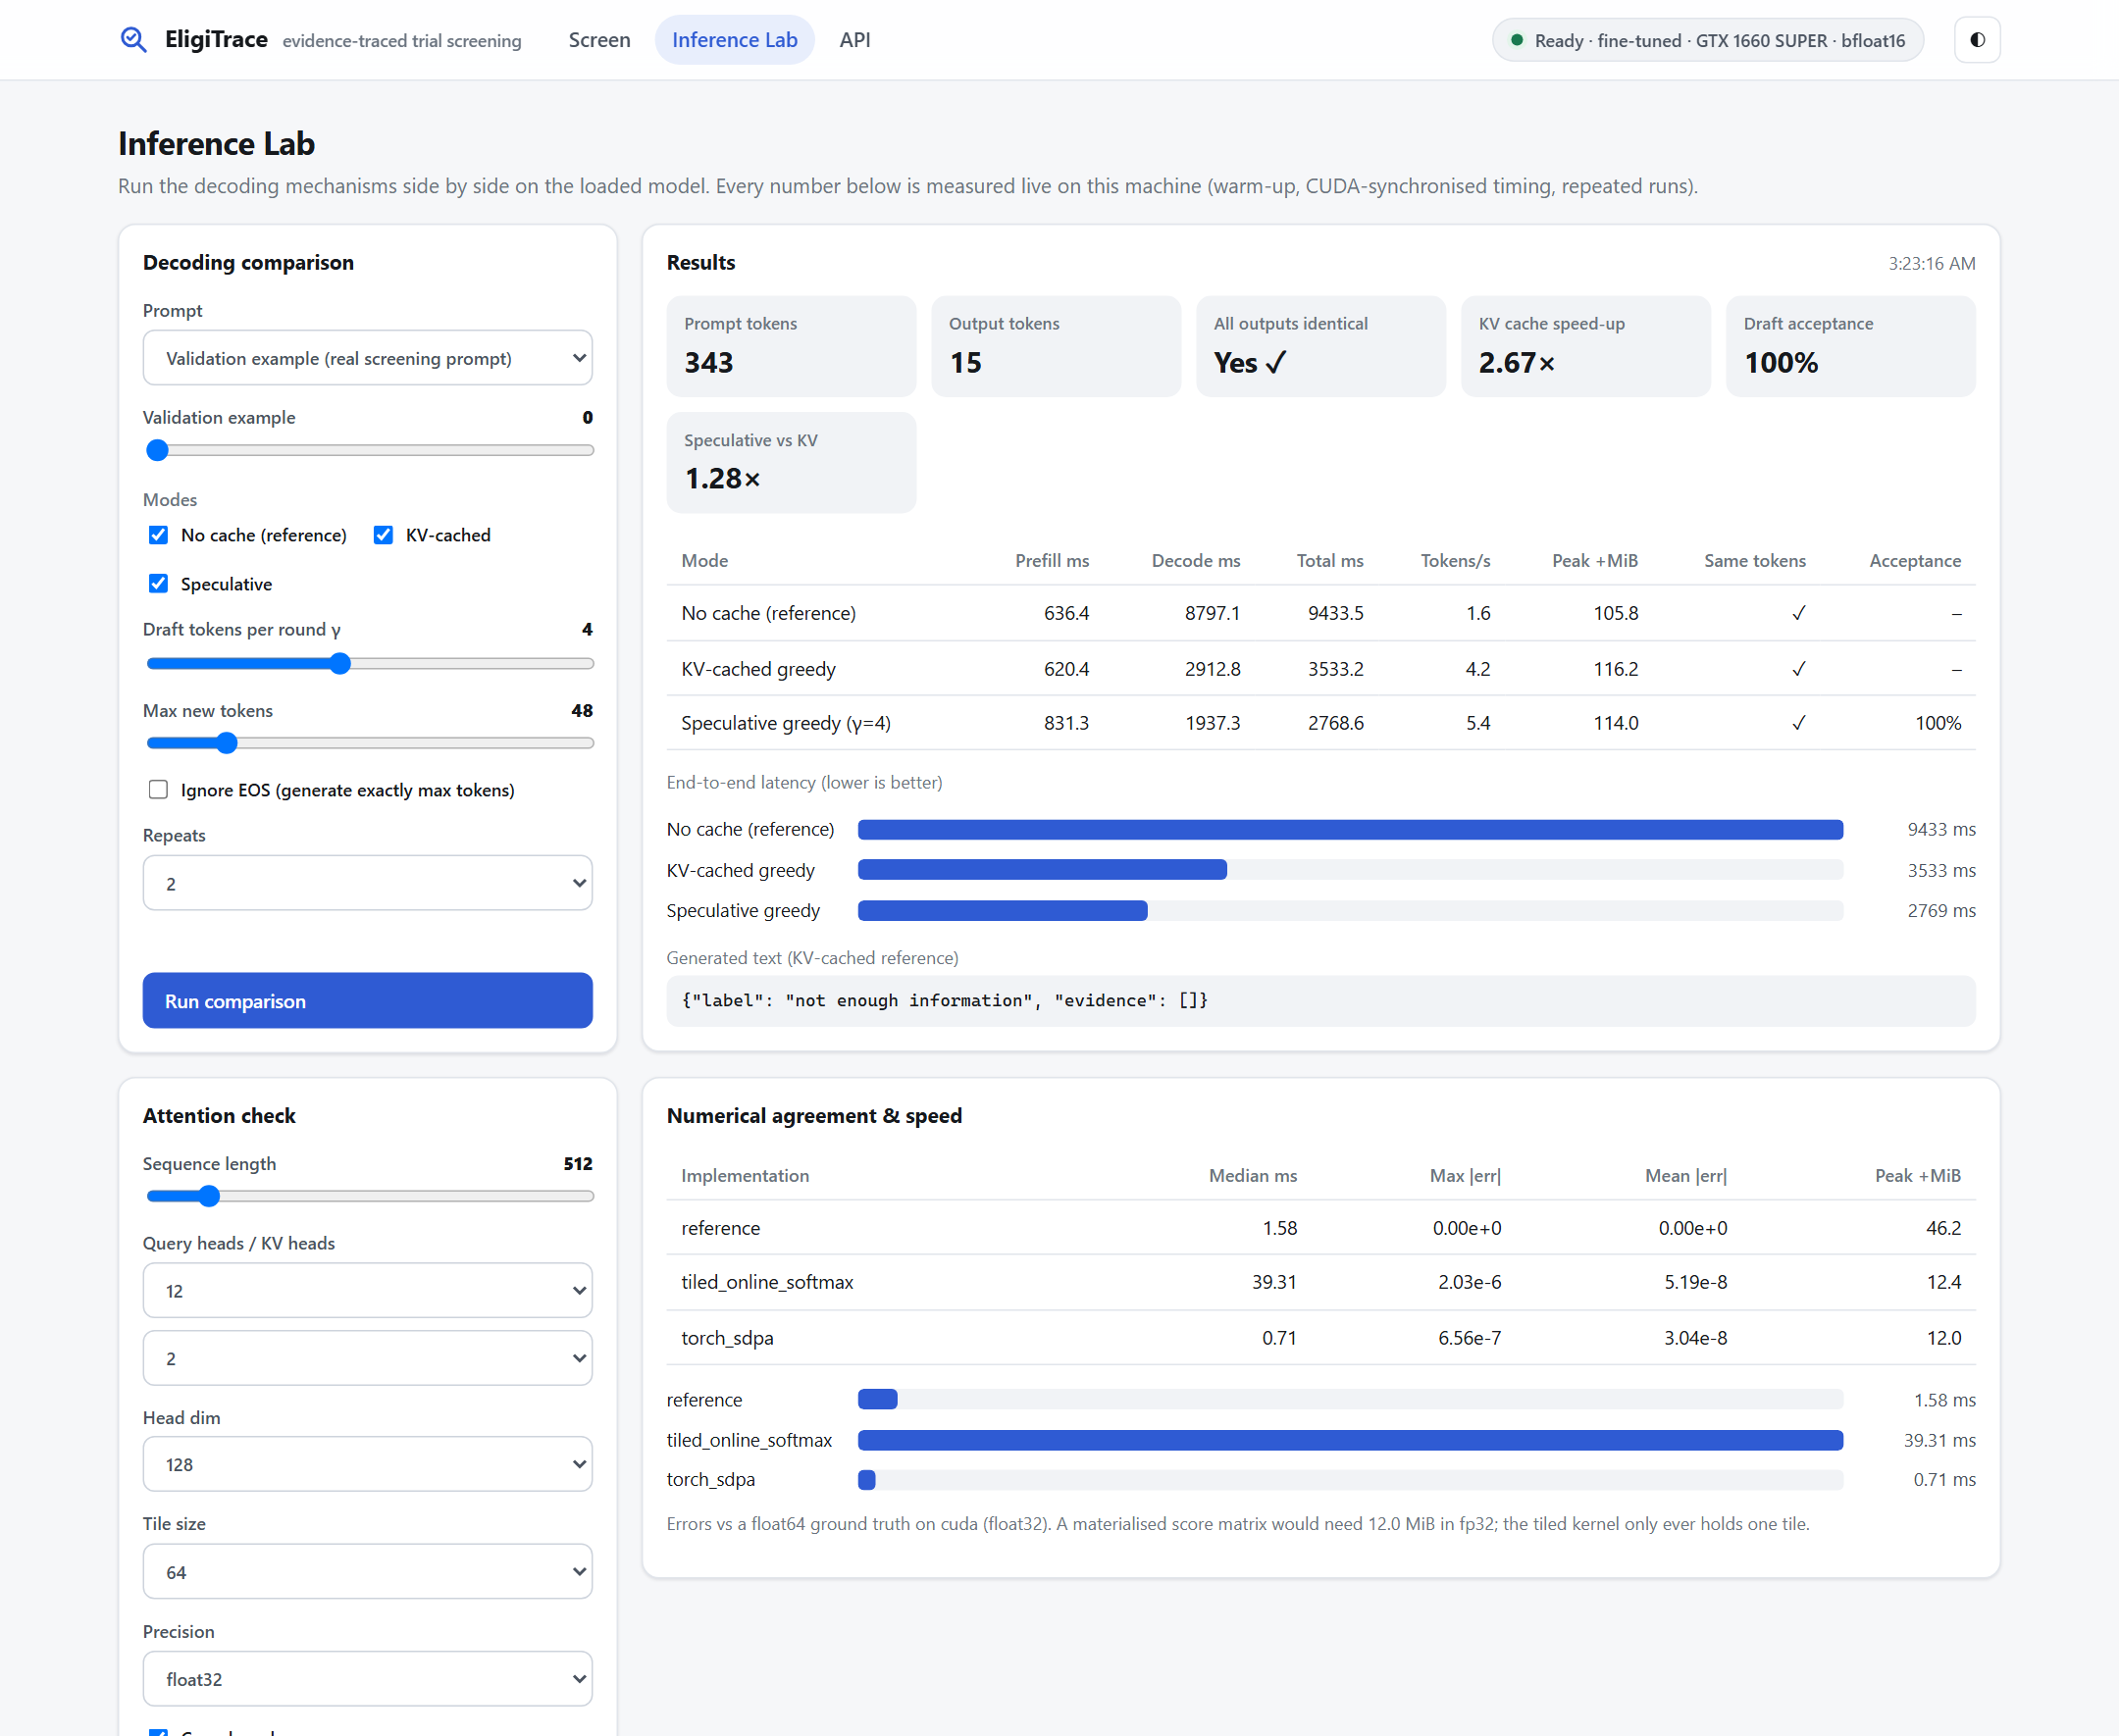
\includegraphics[width=0.49\linewidth]{screens/06_lab.png}\hfill
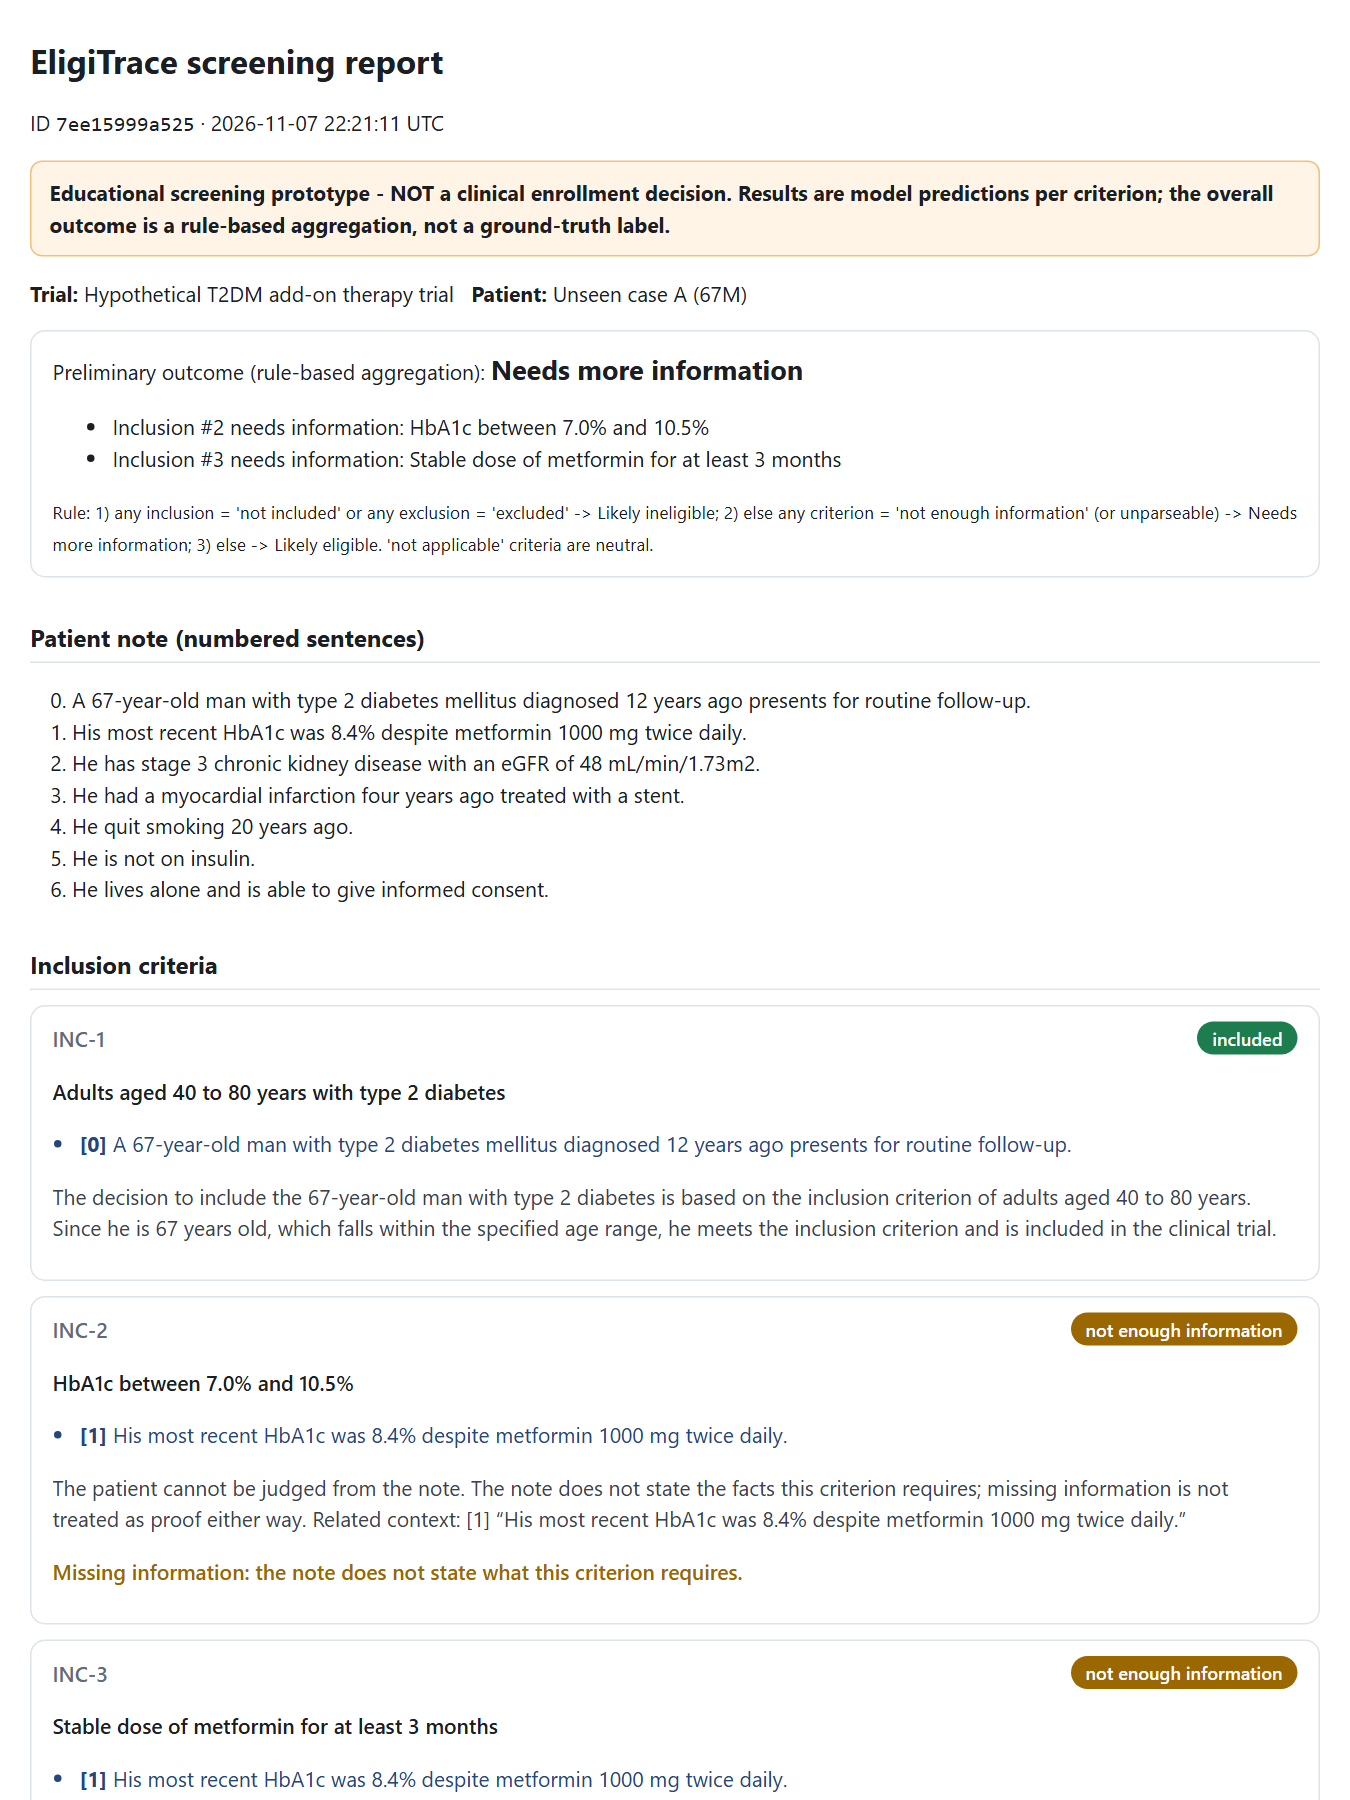
\includegraphics[width=0.49\linewidth]{screens/04_report.png}
\caption{\sys\ application. Top: input of an unseen note and criteria (left), and criterion results with
highlighted evidence, grounded rationales and the rule-based outcome (right). Bottom: Inference Lab with live
decoder and attention comparisons (left), and the exported report with provenance (right).}
\label{fig:app}
\end{figure*}

